\clearpage{\pagestyle{empty}\cleardoublepage}
\chapter{Architettura del sistema}
%
Il sistema di monitoraggio presentato in questa tesi \`e stato progettato 
quale possibile soluzione per una azienda installatrice di impianti fotovoltaici 
su vasta scala.
%

%
Perch\'e una azienda installatrice dovrebbe interessarsi ad un sistema 
di monitoraggio? Le motivazioni possibili sono almeno due:
%
\begin{itemize}
\item l'azienda potrebbe fornire, ai clienti che lo desiderano, un pacchetto 
      comprensivo di impianto fotovoltaico e sistema di monitoraggio; le 
      informazioni prodotte da quest'ultimo potrebbero essere utilizzate 
      per realizzare un sistema informativo in grado di dare visione 
      al cliente \Item{i} dello stato del suo impianto, \Item{ii} del 
      suo rendimento e, quindi, \Item{iii} del ritorno economico 
      rispetto all'investimento effettuato
%
\item una azienda installatrice fornisce una garanzia sull'impianto e, spesso, 
      si occupa anche della manuntenzione di quest'ultimo; un sistema di 
      monitoraggio permetterebbe di tenere sotto costante osservazione 
      lo stato degli impianti installati, a livello di componente; ci\`o
      permetterebbe una previsione e una identificazione da remoto, di 
      eventuali \emph{fault}, andando ad abbattere i costi di manutenzione
      degli impianti
\end{itemize}
%

%
Nel capitolo precendete sono state presentate alcune delle soluzioni di 
monitoraggio proposte in letteratura. Tuttavia, nessuno dei sistemi analizzati 
\`e stato progettato per un impiego su vasta scala da parte di una impresa, 
piuttosto si tratta di sistemi \emph{prototipo}, pensati pi\`u per un uso 
accademico che per la produzione in serie.
%

%%
La progettazione di un sistema di monitoraggio da produrre in serie e da utilizzare su 
vasta scala non pu\`o non tenere conto di fattori quali il costo dei 
componenti, la facilit\`a d'installazione, ecc.
%

%
La fase iniziale della progettazione del sistema oggetto della presente tesi
ha, quindi, visto l'individuazione della seguente lista di \emph{desiderata}:
%
\begin{itemize}
\item \emph{modularit\`a}, i.e. il sistema deve essere composto da vari dispositivi di 
      campo, ciascuno dei quali con una ben precisa responsabilit\`a; il numero e il 
      tipo dei dispositivi da installare dipender\`a, di volta in volta, dalle dimensioni 
      dell'impianto da monitorare
%
\item \emph{bassi costi di produzione}, i.e. il prezzo del sistema da proporre al cliente 
      finale dovr\`a essere \emph{ragionevolmente} pi\`u basso rispetto al costo totale 
      dell'investimento da lui effettuato
%
\item \emph{semplicit\`a di installazione}, i.e. il sistema dovrebbe richiedere una quantit\`a
      di lavoro minimale per il suo setup; tale obiettivo pu\`o essere raggiunto, ad esempio,  
      progettando un sistema che non richieda l'installazione di troppi cavi per 
      l'interfacciamento dei componenti, oppure, ancora, utilizzando dei dispositivi 
      \emph{autoconfiguranti}
%      
\item \emph{indipendenza da una linea dati cablata}, i.e. non tutti gli impianti fotovoltaici
      sono installati in zone urbane, anzi, molti si trovano in zone rurali non raggiunte da linee 
      dati di terra; l'ideale, per un sistema di monitoraggio, sarebbe fare affidamento
      su meccanismo di trasferimento dati via \emph{gsm} e \emph{gprs}.
%
\end{itemize}
%

\section{Panoramica del sistema}
%
L'architettura generale del sistema realizzato \`e rappresentata in figura 
\ref{architettura-sistema}.
%
\begin{figure}[!h]
\centering
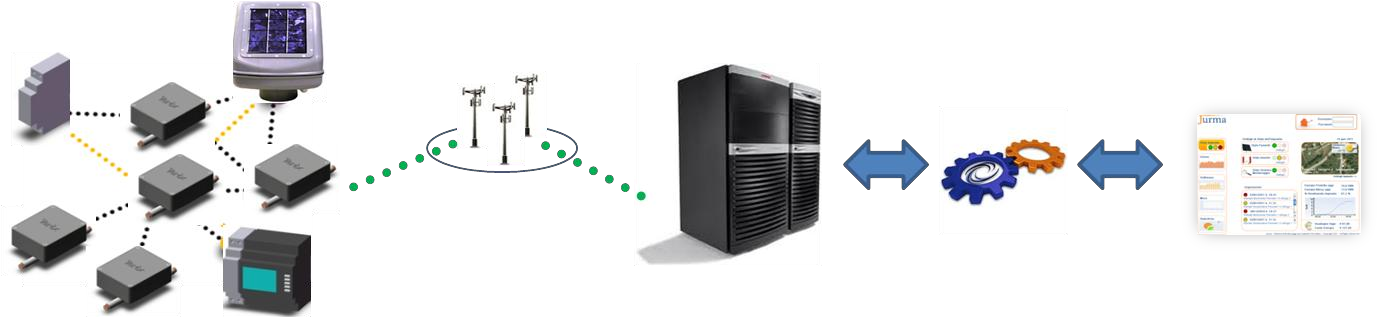
\includegraphics[width=400pt]{img/architecture.png}
\caption{Architettura del sistema}
\label{architettura-sistema}
\end{figure}
%
Nella parte sinistra, \`e presente l'infrastruttura di sensori di campo 
utilizzata per la misura delle grandezze rilevanti.
%
Tale infrastruttura trasmette le letture rilevate mediante una connessione dati 
gprs o gsm ad un \emph{datacenter}, il cui compito \`e quello di processare i dati 
ricevuti, produrre report e allarmi, e pubblicare tutto ci\`o mediante dei 
\emph{web services}.
%
Infine, nella parte pi\`u a destra della figura, \`e rappresentato il \emph{portale web} 
che, utilizzando i servizi web esposti dal datacenter come sorgente dati, fornisce 
una rappresentazione visuale e interattiva dei dati prodotti dal sistema.
%

%
Cominciamo l'analisi del sistema dalla infrastruttura dei sensori di campo.
%
In particolare, vediamo quali grandezze si \`e scelto di misurare e quali sono
state le scelte tecnologiche per la realizzazione della infrastruttura.
%

%
\section{Grandezze rilevanti}
\label{sec:grandezze-rilevanti}
%
La classificazione degli utenti proposta in \cite{kolodenny08} pu\`o essere utile ai 
fini dell'individuazione delle grandezze rilevanti. Le esigenze di monitoraggio 
espresse nell'introduzione a questo capitolo, infatti, prevedono che il sistema 
sia in grado di produrre sia le informazioni cui tipicamente sono interessati i 
\emph{proprietari} degli impianti, sia le informazioni utili ai \emph{manutentori} 
per rilevare malfunzionamenti ed, eventualmente, effettuare diagnosi.
%

%
Alla luce di ci\`o, sono state individuate come rilevanti per un generico impianto 
caratterizzato dalla seguente configurazione,
%
\begin{itemize}
\item $NI$, numero di inverter.
\item $NS_k, k \in \{1, \dots, NI\}$, numero di stringhe dell'inverter $k$.
\item $\eta _{k}, k \in \{1, \dots, NI\}$, rendimento in potenza
  dell'inverter $k$ (rapporto tra
  potenza in uscita e potenza in ingresso).
\item $NP_{j,k}, k \in \{1, \dots, NI\}, j \in \{1, \dots, NS_k\}$, numero
  di pannelli della stringa $j$ legata all'inverter $k$.
\item $\mu _{i,j,k}, k \in \{1, \dots, NI\}, j \in \{1, \dots, NS_k\}, i \in
  \{1, \dots, NP_{j,k}\}$, rendimento in potenza del pannello $i$ della stringa
  $j$ dell'inverter $k$ (rapporto tra  potenza in uscita e irraggiamento).
\item $S _{i,j,k}, k \in \{1, \dots, NI\}, j \in \{1, \dots, NS_k\}, i \in
  \{1, \dots, NP_{j,k}\}, (m^2)$, Superficie del pannello $i$ della stringa
  $j$ dell'inverter $k$.
\end{itemize}
%
le grandezze definite nel seguente \emph{schema}, il quale non si limita ad elencarle, 
ma definisce anche quali grandezze si \`e deciso di misurare direttamente e 
quali, invece, si \`e deciso di stimare:
%
\begin{enumerate}
%%
\item Dati Ambientali:
\begin{itemize}
\item $T, (\deg C)$, Temperatura ambiente.
\item $R, (W/m^2)$, Irraggiamento.
\end{itemize}
%%
%%
\item Grandezze da \textbf{misurare} a monte del contatore bidirezionale:
\begin{itemize}
%%
\item$E_O, (KWh)$, Energia attiva totale prodotta.
\item$P_O, (KW)$, Potenza attiva.
\item$PR_O, (KW)$, Potenza reattiva.
\item$V_O, (V)$, Tensione.
\item$I_O, (A)$, Corrente.
\item$PF_O, (adimensionale)$, Sfsamento (power factor o $cos \phi$).
%%
\end{itemize}
%%
%%
\item Grandezze da \textbf{misurare} a valle dell'inverter $k$:
\begin{itemize}
%%
\item$Iout_{k}, (A)$, Corrente generata.
%%
\end{itemize}
%%
%%
\item Grandezze da \textbf{stimare} per l'inverter $k$:
\begin{itemize}
%%
\item$Vout_{k} = V_O, (V)$, Tensione generata.
\item$Pout_{k} = Vout_{k} \cdot Iout_{k}  \cdot PF_O, (KW)$ Potenza
  (attiva) generata
\item$Pin_{k} = \frac{Pout_k}{\eta _k}, (KW)$, Potenza in ingresso
  all'inverter generata dalle stringhe.
%%
\item$Vin_{k} = \frac{Pin_k}{\sum_{j=1}^{NS_k}{Is_{j, k}}}, (V)$, Tensione
  in ingresso all'inverter
  calcolata sulla base della corrente prodotta dalle stringhe.
%%
\end{itemize}
%%
%%
\item Grandezze da \textbf{misurare} a valle della stringa $j, k$:
\begin{itemize}
%%
\item$Is_{j, k}, (A)$, Corrente generata dalla stringa.
%%
\end{itemize}
%%
%%
\item Grandezze da \textbf{stimare} per la stringa $j, k$:
\begin{itemize}
%%
\item$Vs_{j, k} = Vin_{k}, \forall k, (V)$, Tensione generata da ogni stringa.
\item$Ps_{j, k} = Vs_{j,k} \cdot Is_{j,k}, (KW)$, Potenza generata da ogni
  stringa.
%%
\end{itemize}
\end{enumerate}
%

%
Come vedremo in seguito, tale schema \`e assolutamente \emph{generico}. 
%
La modularit\`a che caratterizza il sistema implementato permette, infatti, 
di scegliere tra due possibili \emph{profili di monitoraggio}: uno \emph{basic}, 
pi\`u economico, che si limita alla sola misurazione della potenza scambiata con 
la rete al fine di monitorare la produzione energetica dell'impianto (tale soluzione 
\`e ideale nel caso di impianti di piccola dimensione) e uno \emph{pro}, che effettua 
la misurazione di tutte le grandezze riportate nello schema (ed \`e pi\`u adatto a 
impianti di grandi dimensioni, dove diagnosticare un malfunzionamento richiede 
una conoscenza di livello pi\`u approfondito dello stato dell'impianto).
%

%
\section{Dispositivi di campo}
Per la misura delle grandezze rilevanti, si \`e deciso di seguire l'approccio
proposto in \cite{xiaoli11}, ovvero l'implementazione di una WSN basata 
su ZigBee. 
%
Questo tipo di soluzione \`e particolarmente adatta alle nostre esigenze, 
in quanto non prevede alcun tipo cablaggio; inoltre, i transponder 
ZigBee sono noti per i loro profili di consumo \emph{ultra-low power}: 
ci\`o permette di alimentare i dispositivi con batterie al litio per un periodo 
di tempo dell'ordine degli anni, e, quindi, permette ai dispositivi di essere
totalmente indipendenti da fonti di alimentazione esterna; per le WSN ZigBee, inoltre, 
esistono dei profili applicativi che prevedono il \emph{set up} automatico, 
ovvero l'autoconfigurazione, della WSN, senza alcuna necessit\`a di intervento 
umano.
%

%
Per effettuare le misurazioni, sono stati previsti due tipi di dispositivi di 
campo: \emph{power/inverter transponders}, e \emph{string transponders}.
%
Un terzo tipo di componente, il \emph{gateway}, funger\`a da \emph{coordinatore}
della WSN e da \emph{concentratore} dati, i.e. interrogher\`a a turno ciascuno
dei nodi della WSN e invier\`a i dati di campo raccolti al datacenter mediante 
gsm o gprs.
%

%
\subsection{Gateway}
%
Come anticipato, il \emph{Gateway} costituisce il \emph{coordinatore} della 
WSN formata dai dispositivi di campo.
%
In quanto tale, si occupa di raccogliere le misure effettuate dai sensori 
e di trasmetterle al datacenter.
%
\begin{figure}[!h]
\centering
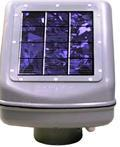
\includegraphics[width=100pt]{img/gw.jpg}
\caption{Gateway}
\label{gw}
\end{figure}
%

%
Come visibile dalle figure \ref{gw} e \ref{gw-opened}, il dispositivo \`e composto 
da un insieme di componenti integrati, che includono, tra gli altri,  \Item{i} il 
modem gsm/gprs, \Item{ii} il transponder radio ZigBee, \Item{iii} la batteria, 
\Item{iv} un fusibile per l'attivazione della rete wireless e \Item{v} un 
piccolo modulo fotovoltaico sulla cover.
%
Tale elemento \`e funzionale sia alla ricarica delle batteria, sia alla stima
del valore di irraggiamento sul campo.
%
\begin{figure}[!h]
\centering
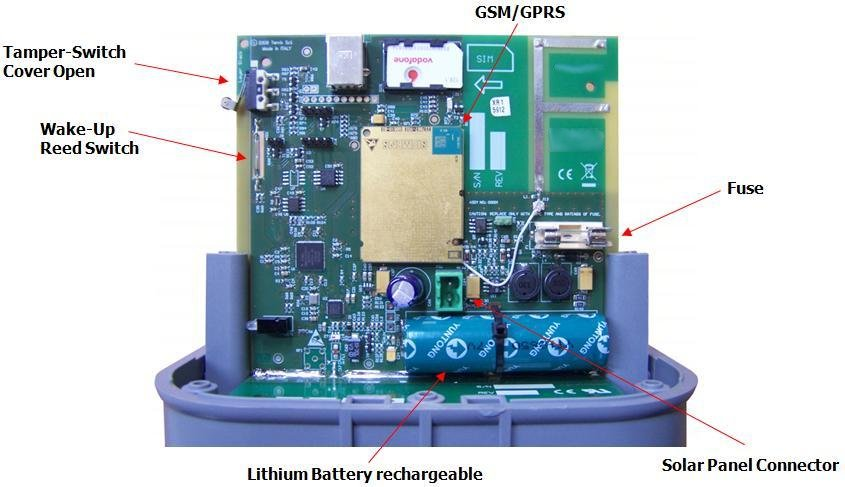
\includegraphics[width=350pt]{img/gw-opened.jpg}
\caption{Elettronica interna del gateway}
\label{gw-opened}
\end{figure}
%

%
Il gateway effettua l'interrogazione dei dispositivi di campo ad intervalli 
predefiniti; la durata dell'intervallo pu\`o essere configurata da remoto, a seconda 
delle esigenze di monitoraggio, i.e. a seconda del rate di campionamento
delle grandezze rilevanti desiderato.
%

%
Una volta raccolte, le misure di campo vengono memorizzate in una memoria locale, 
ed inviate periodicamente al datacenter.
%
La modalit\`a predefinita di trasferimento utilizza una connessione gprs, ed
in particolare, il protocollo FTP, tuttavia, per operare in aree non coperte da 
connettivit\`a gprs, il dispositivo pu\`o essere impostato in modo da trasferire 
i dati tramite via SMS.
%

%
\subsection{Power/Inverter Transponder}
%
Il \emph{Power/Inverter Transponder} \`e un dispositivo costituito da \Item{i} un 
analizzatore di rete e \Item{ii} un transponder ZigBee.
%
Questi dispositivi sono stati pensati per essere collegati alla rete in alternata 
dell'impianto fotovoltaico e, in particolare, per misurare le grandezze rilevanti 
a monte del contatore bidirezionale (power transponder) e a valle degli inverter 
(inverter transponder).
%

%
Il modello di analizzatore di rete scelto \`e il \emph{Socomec Diris A10}
\cite{dirisa10}, in grado di misurare tensione, corrente, potenza, power factor 
e frequenza sia su linee monofase che trifase.
%
\begin{figure}[!h]
\centering
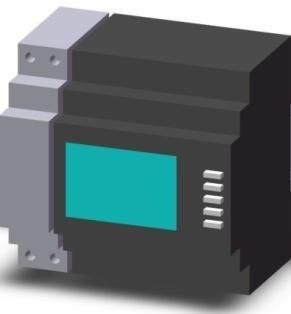
\includegraphics[width=150pt]{img/power-transponder.jpg}
\caption{Socomec Diris A10}
\label{power-transpoder}
\end{figure}
%

%
Gli analizzatori di rete, in genere, non vanno collegati direttamente alle linee di 
potenza su cui effettuare le misurazioni, ma vengono interfacciati mediante dei 
\emph{trasformatori amperometrici} (TA).
%
\begin{figure}[!h]
\centering
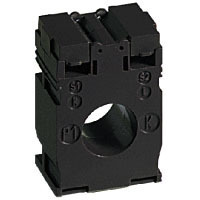
\includegraphics[width=120pt]{img/ta.jpg}
\caption{Trasformatore amperometrico 100/5A}
\label{ta}
\end{figure}
%

%
Essendo dei dispositivi atti alla misura di grandezze di rete in ambito industriale, 
sia gli analizzatori di rete Socomec, sia i TA sono dotati di apposito \emph{attacco} 
per montaggio su barra DIN: ci\`o fa del \emph{quadro di alternata} dell'impianto 
il luogo ideale per l'installazione dei power/inverter transponder.
%

%
\subsection{String Transponder}
%
\begin{figure}[!h]
\centering
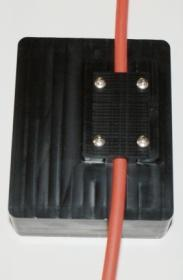
\includegraphics[width=150pt]{img/string-transponder.jpg}
\caption{String Transponder}
\label{string-transponder}
\end{figure}
%
Lo \emph{String Transponder} \`e il dispositivo pensato per la misura delle correnti 
di stringa. \`E anch'esso, come il power/inverter transponder, un dispositivo composito:
\`e costituito da un transponder ZigBee e da un sensore di corrente a \emph{effetto Hall}.
%

%
La scelta dei sensori di corrente induttivi \`e, ancora una volta, frutto della 
necessit\`a di massimizzare la semplicit\`a di installazione del sistema. 
%
Come mostrato in figura \ref{string-transponder}, infatti, l'utilizzo di questi dispositivi
richiede solo che il cavo su cui misurare la corrente venga fatto passare all'interno 
del sensore, senza alcuna necessit\`a di interrompere il cavo stesso.
%

%
\section{Profili di monitoraggio}
%% profili di monitoraggio
%% introduzione al datacenter
